%--------------------------------------------------------------------
\section{Implementations}
\label{impl}

Fresnel has been designed as an application- and output format-independent RDF presentation vocabulary. In this section we give an overview of various applications implementing Fresnel: Longwell \cite{simile} and Horus \cite{horus} which both render RDF data as HTML Web pages using nested box layouts, IsaViz \cite{isaviz} which represents RDF graphs as node-link diagrams, and Cardovan, a browser and lens editor based on the SWT GUI toolkit.

\vspace{1em}
{\bf Longwell} is a Web-based RDF browser whose foundational navigation paradigm is faceted browsing. Faceted browsing displays only the properties that are configured to be 'facets' (i.e., to be important for the user browsing data in one or more specific domains) using values for those fields as a means for zooming into a collection by selecting those items with a particular field-value pair.

\begin{figure}
\begin{center}
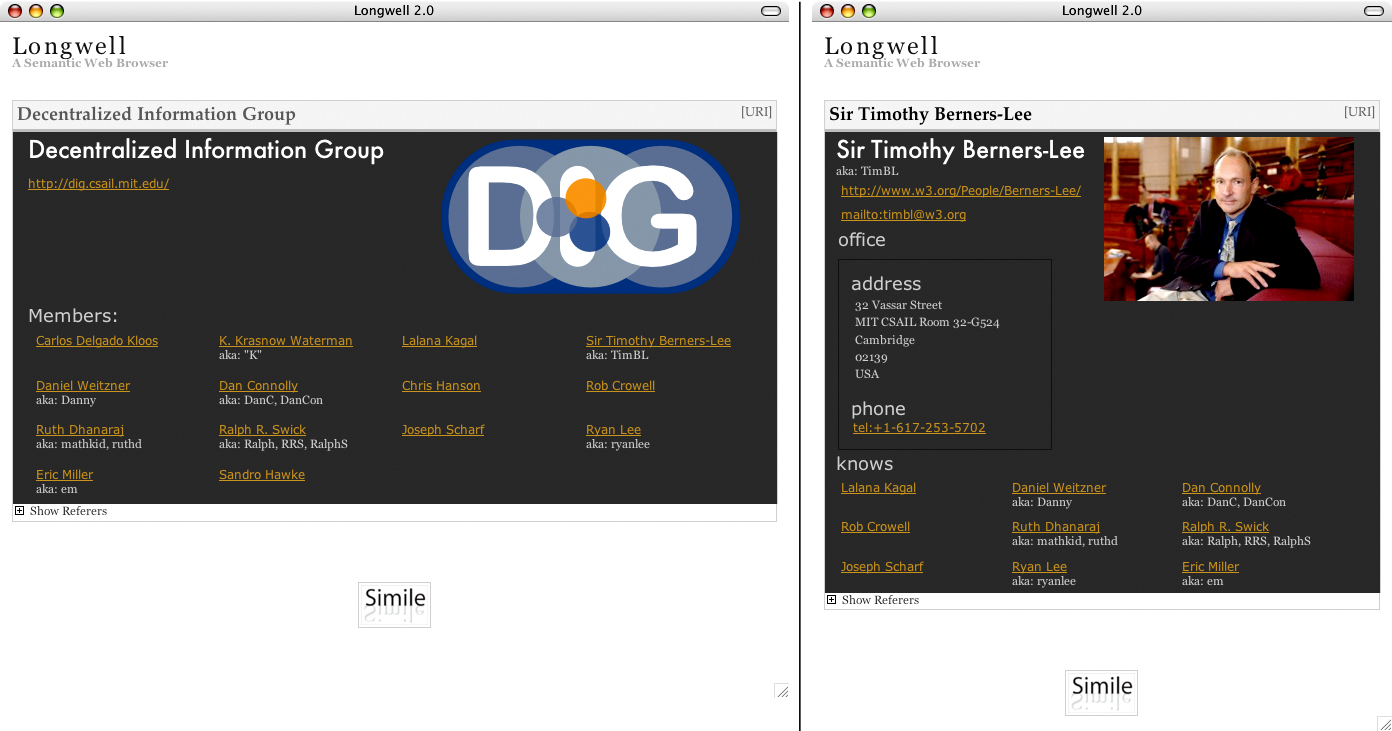
\includegraphics[width=12cm]{longwellScreens.png}
\end{center}
\vspace{-2em}
\caption{Displaying a view of an organization (left) and a constituent member (right) in Longwell}
\label{longwellFig1}
\vspace{-1em}
\end{figure}

The latest version of Longwell relies on the SIMILE Fresnel rendering engine, a Java library built on the Sesame triple store. The engine implements all of the Fresnel core vocabulary and the portion of the extended vocabulary relating to linking groups to CSS stylesheets as well as the option of using FSL as a selector language.
% The emphasis of the Fresnel engine is on building a correct implementation. 
The Fresnel engine output consists solely of an XML representation of the Fresnel lenses and formats as they apply to one resource. Longwell then applies an XSLT transformation to the XML to generate XHTML.  The default XSLT stylesheet shipped with Longwell will generate a traditional nested box layout, as Horus does, but the stylesheet can be modified by XSLT developers to change the model as they see fit.

The left side of Figure \ref{longwellFig1} shows the rendering of a \rdf{foaf:Organization} resource using a lens that gives some details about the organization and lists its constituent members, all \rdf{foaf:Person}s, each listed with their corresponding nickname information to assist in identification.

The nickname list for each person is preceded by the string 'aka: ', added to the display by using the \rdf{fresnel:contentFirst} directive.  The list is also comma separated, accomplished by setting \rdf{fresnel:contentAfter} to a comma.  Clicking on a URI in the display brings the user to that URI; clicking on a textual label changes Longwell's focus to the resource represented by that label.

On the right side of Figure \ref{longwellFig1}, the focus is on one specific member of the organization featured in the left side.  A sublens is used to generate office contact details, and the same sublens used in the organization focus (left image) to describe an organization's members is used in the person focus (right image) to describe who this person claims to know.


\vspace{1em}
{\bf Horus} is an RDF browser that displays RDF information using a nested box layout. The browser provides a simple navigation paradigm for selecting RDF resources and allows users to switch between different lenses for rendering the resources. Horus supports Fresnel lenses and formats, which can be associated together using Fresnel groups. Groups can refer to external CSS style sheets which are used to define fonts, colors and borders. Horus supports basic selectors, but does not offer SPARQL and FSL as selector languages. Horus is implemented using PHP and is backed by a MySQL database. Applying a lens to an RDF resource results in an intermediate tree, which is formatted afterwards using the formats that are associated to the group of the selected lens. The ordered and formatted intermediate tree is then serialized into XHTML.  

\begin{figure}
\begin{tabular}{cc}
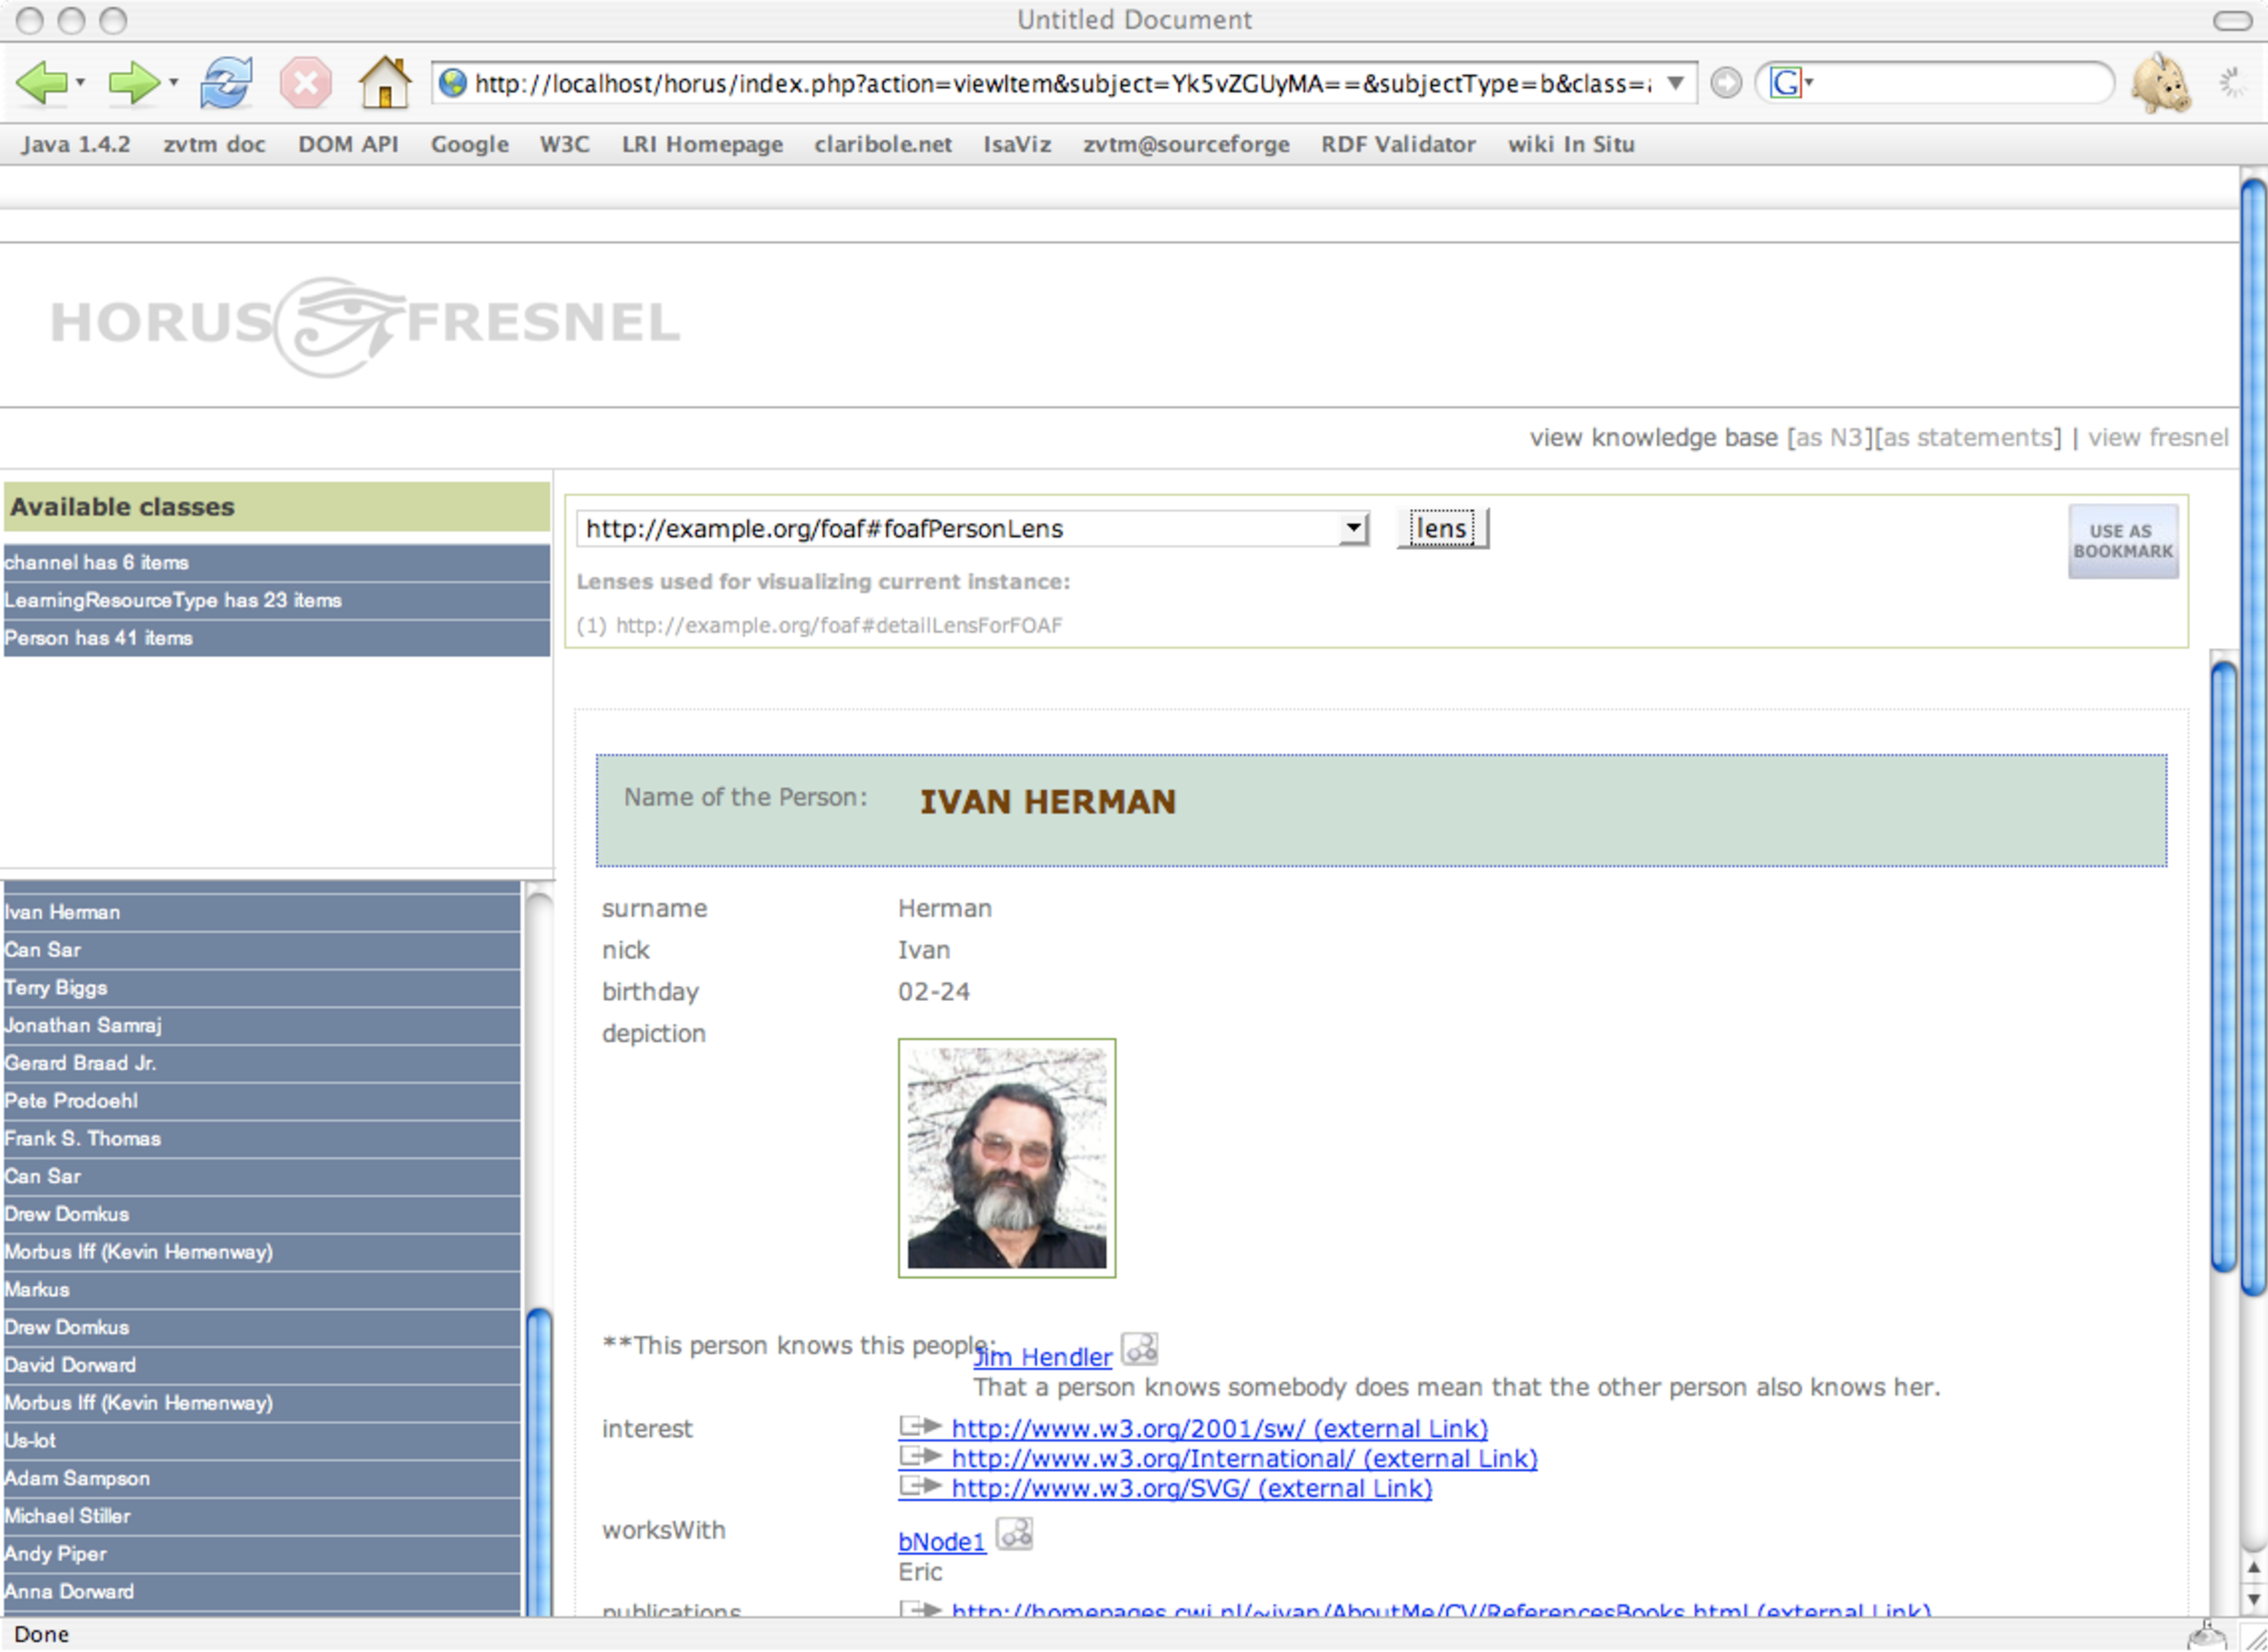
\includegraphics[width=6cm]{horus1.pdf} \hspace{0.02cm} &
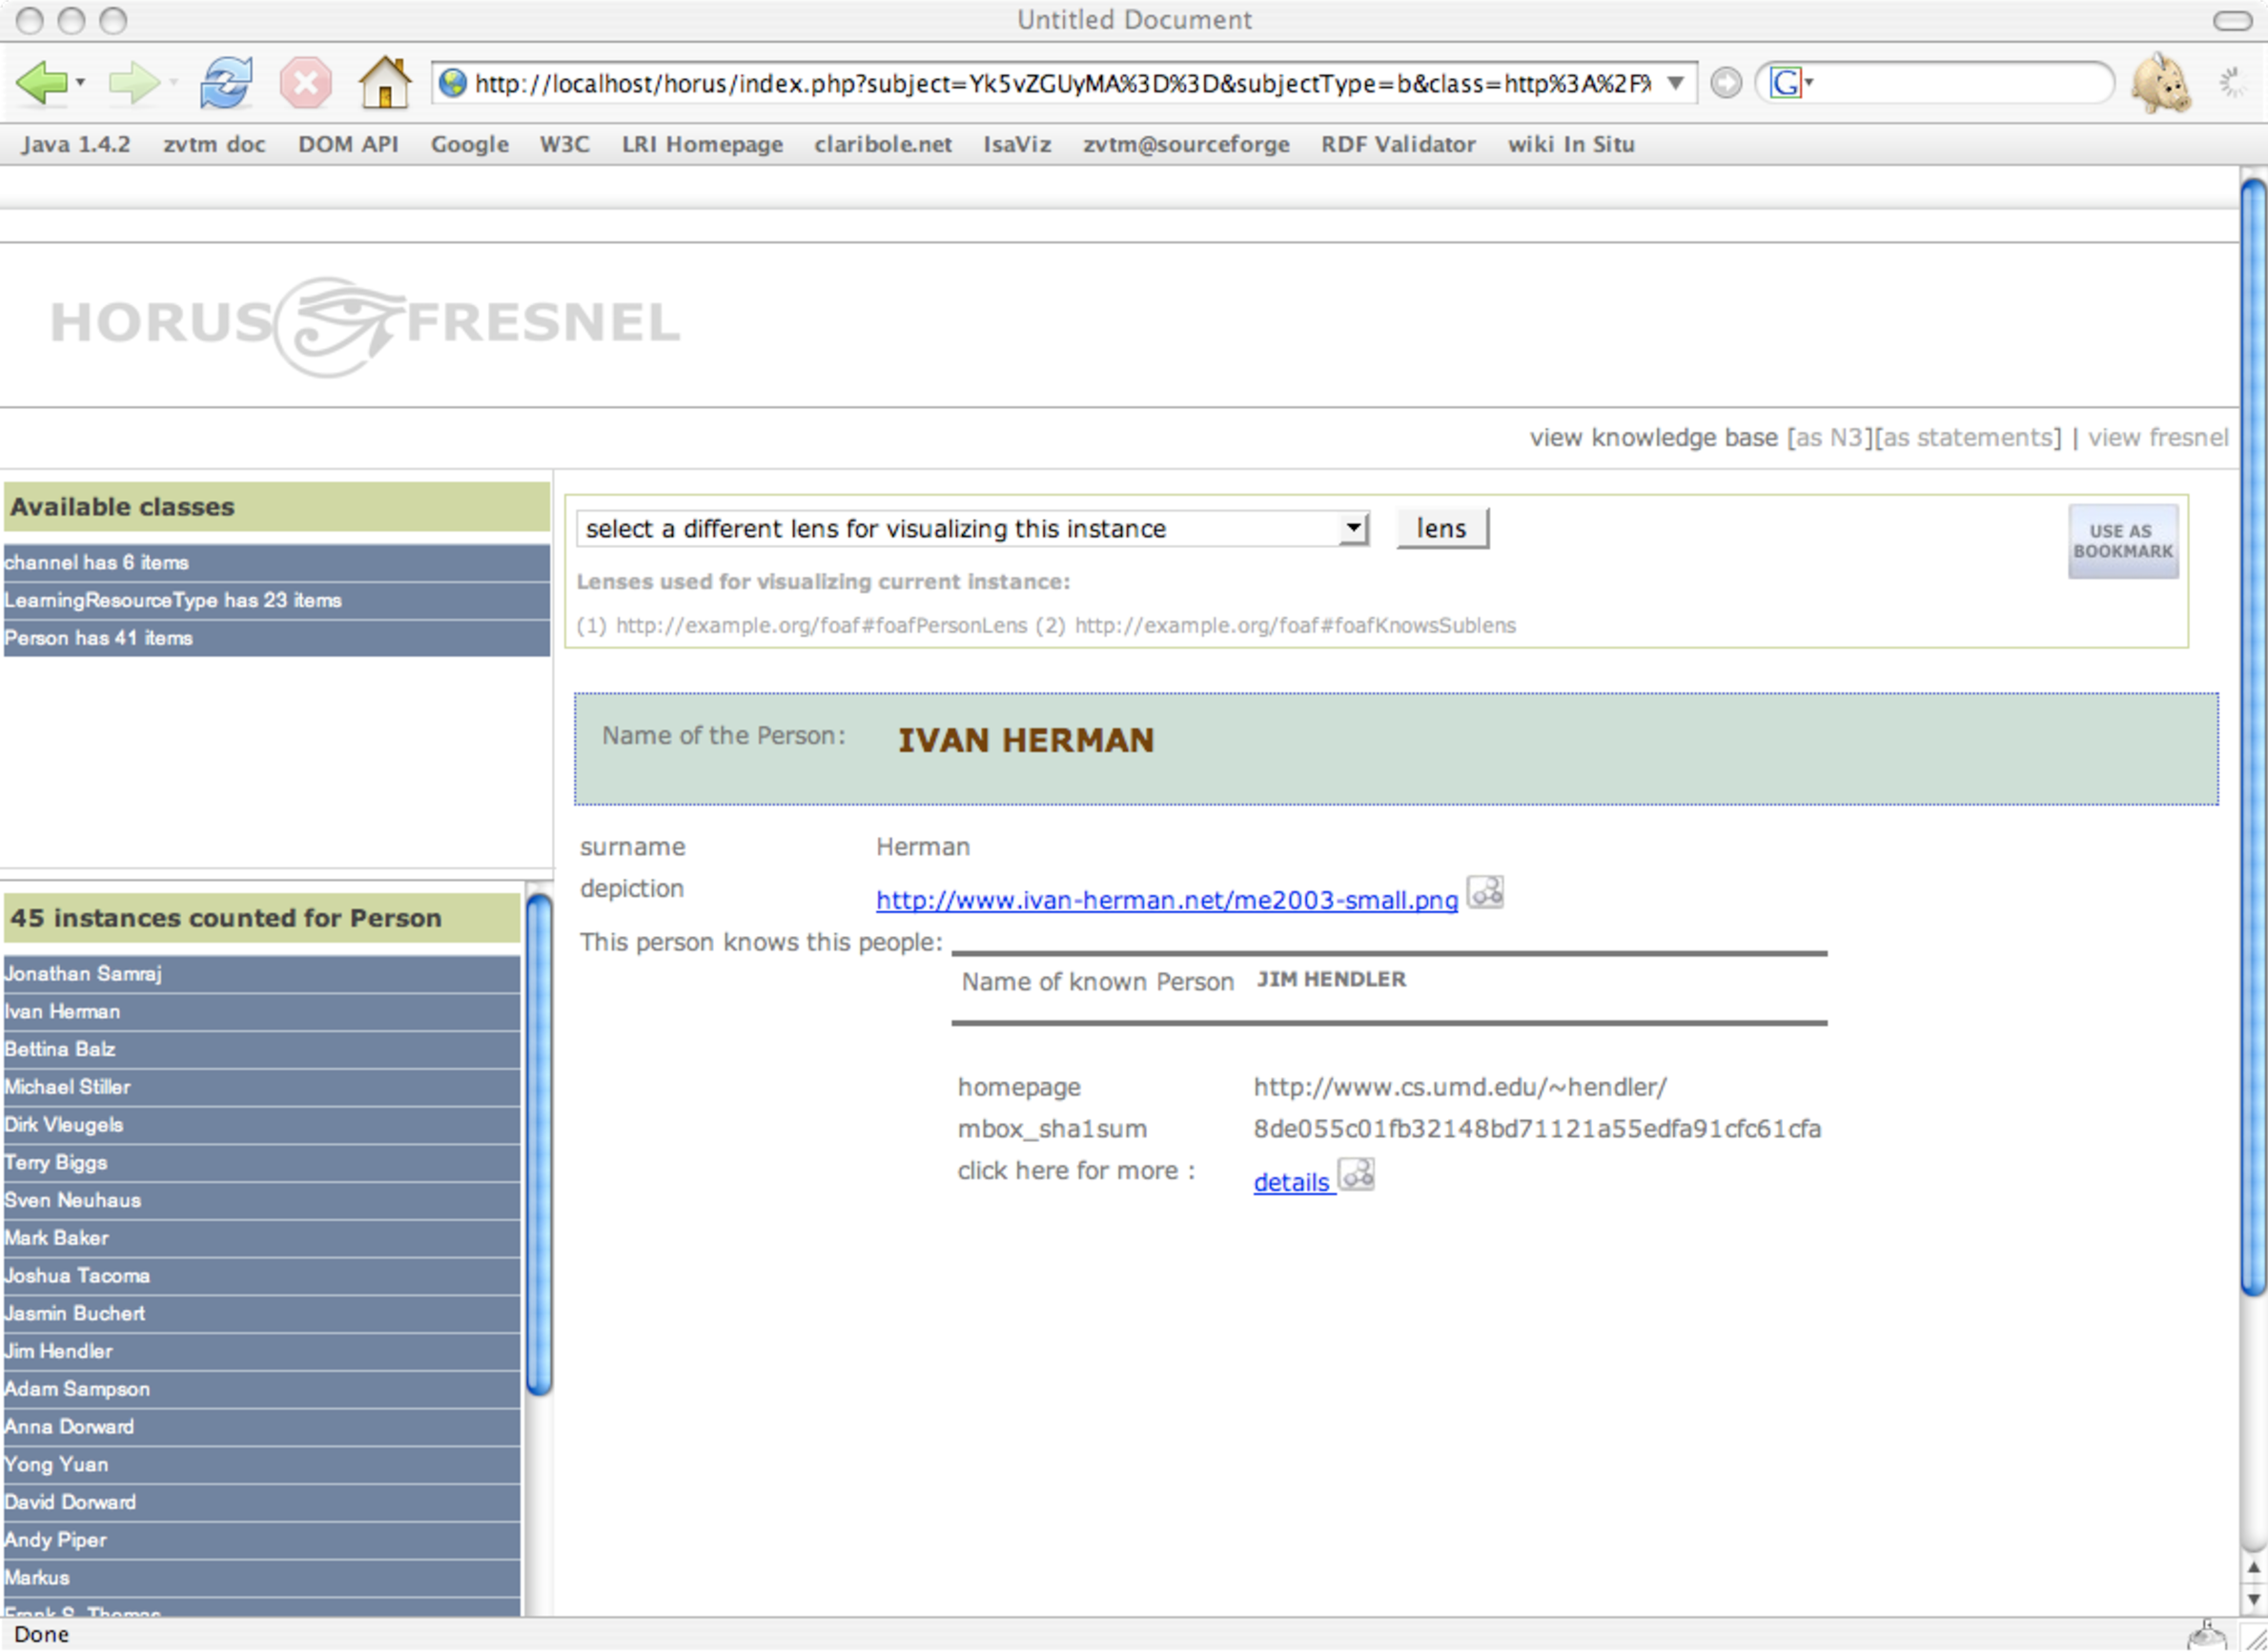
\includegraphics[width=6cm]{horus2.pdf} \\
\end{tabular}
\vspace{-1em}
\caption{Two different views on the same person in Horus: detailed view (left), friends view (right)}
\label{horusFig1}
\vspace{-1.1em}
\end{figure}

Figure \ref{horusFig1} shows two different views on the same person in Horus. The view on the left uses a lens that displays many details about persons. The sentence "{\em This person knows the following people}" is a custom label for property \rdf{foaf:knows}. The disclaimer "{\em That a person knows somebody does\ldots}" is static content added using property \rdf{fresnel:contentLast}. Some of the links are formatted as external links (\rdf{fresnel:value} formatting instruction set to \rdf{fresnel:externalLink}), while others refer to RDF resources in the knowledge base, and thus have a different rendering.

%\begin{figure}
%\begin{center}
%\begin{tabular}{c}
%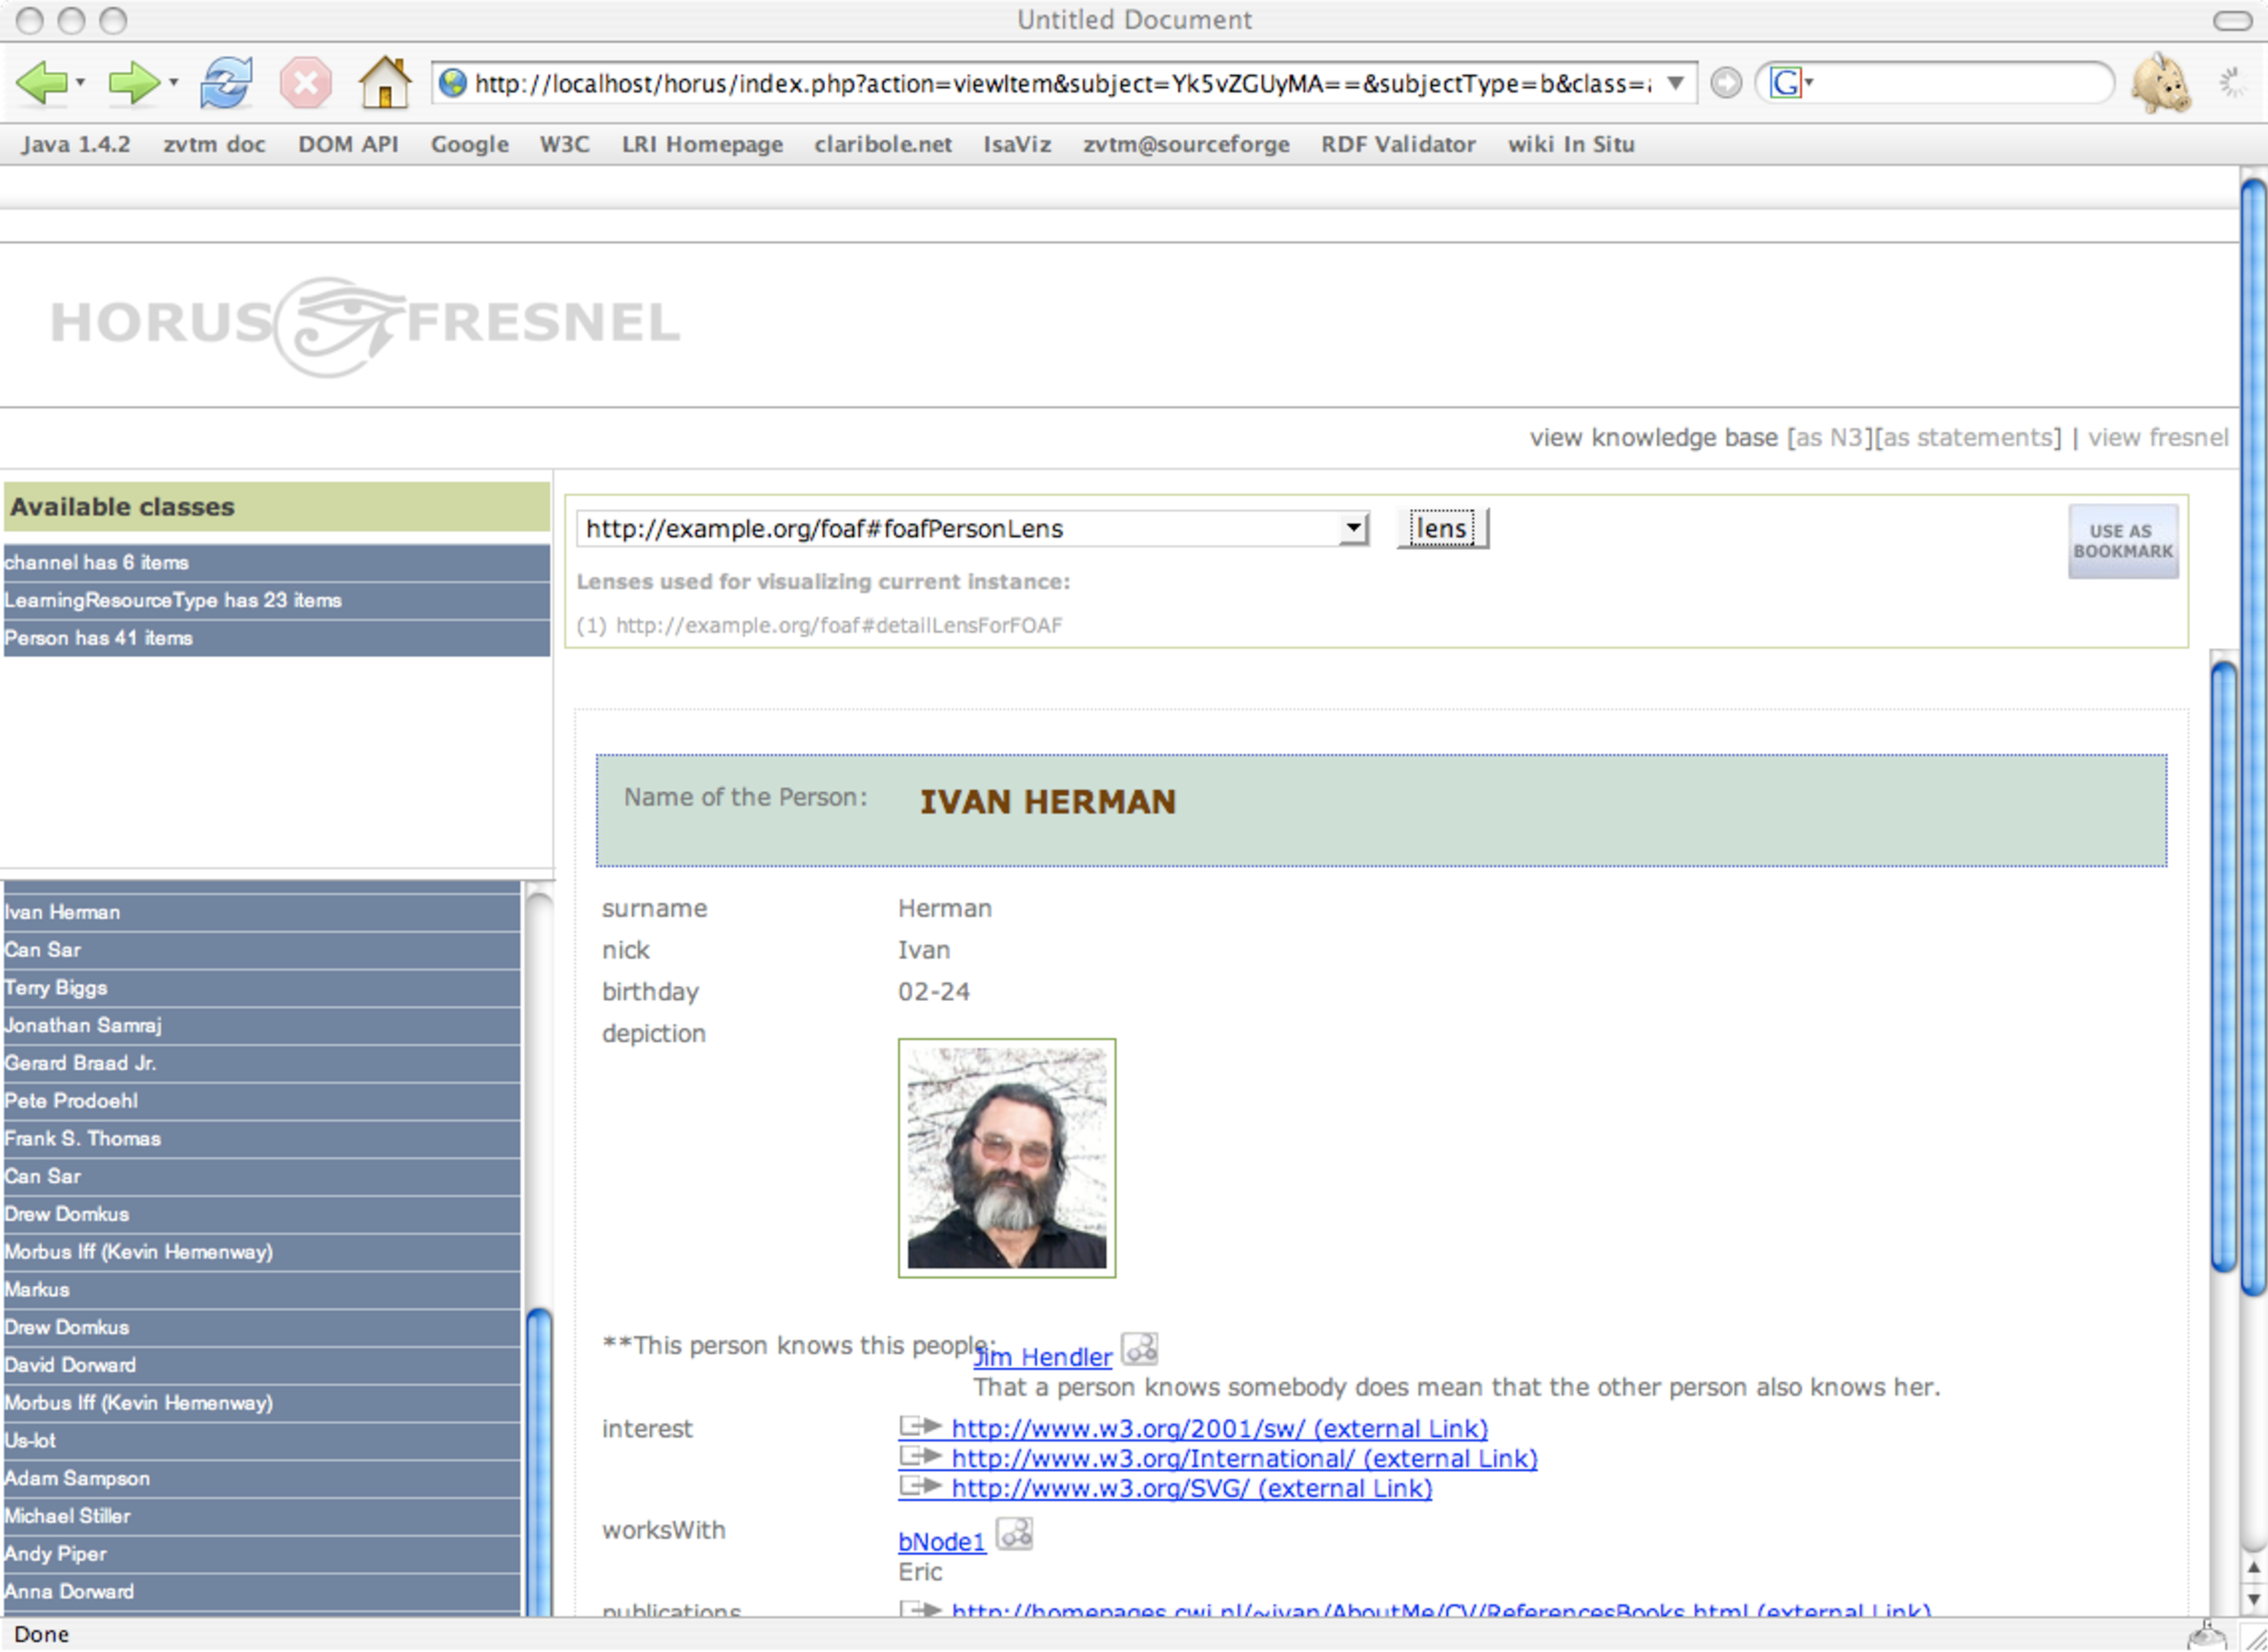
\includegraphics[width=10cm]{horus1.pdf} \\
%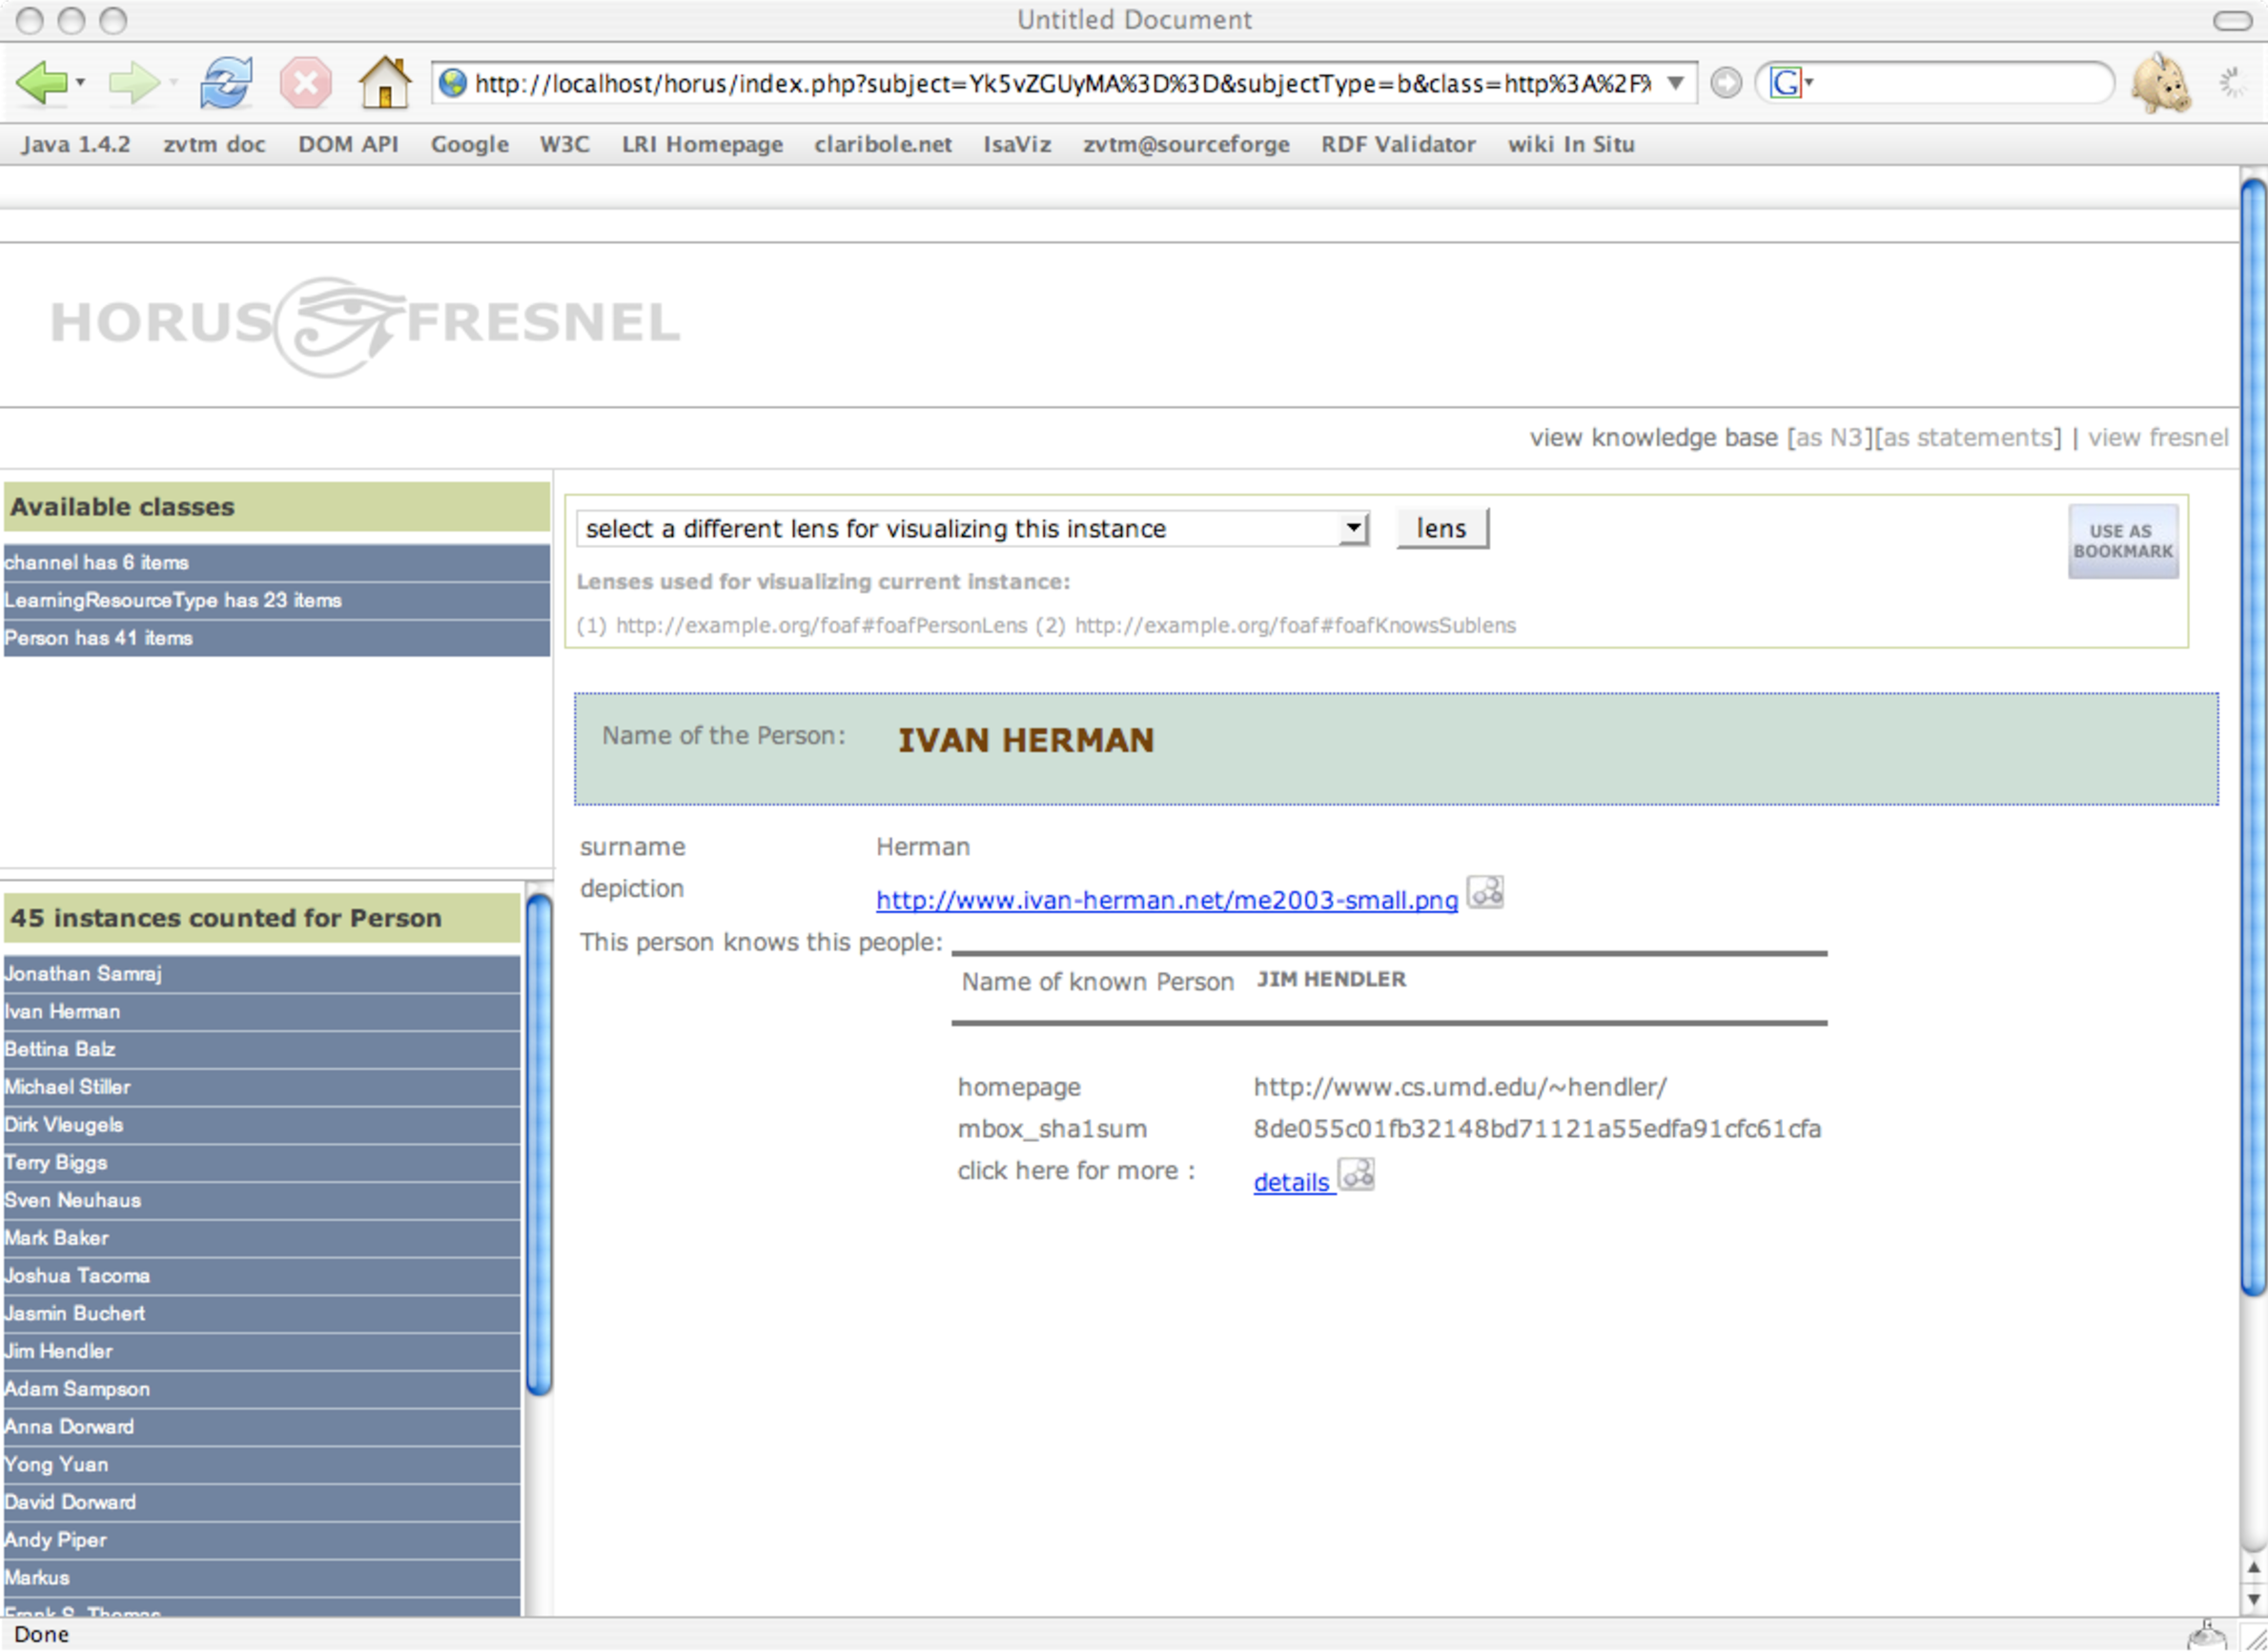
\includegraphics[width=10cm]{horus2.pdf}
%\end{tabular}
%\end{center}
%\caption{Two different views on the same person in Horus: detailed view (left), friends view (right)}
%\label{horusFig1}
%\end{figure}


On the right side of Figure \ref{horusFig1}, the same person is shown using a different lens. This lens displays less details about the person itself, but refers to a second lens (used as a sublens) for displaying details about other persons known by this person. As the sublens belongs to a different group, another CSS class is used to style the names of the person's friends.


\vspace{1em}
{\bf IsaViz} is an RDF authoring environment representing RDF models as node-link diagrams. The interpretation of Fresnel in IsaViz is inspired by both Generalized Fisheye Views \cite{furnas06} and Magic Lenses \cite{bier93}. Fresnel lenses, in conjunction with the formats associated with them through groups, are considered as ``genuine'' lenses that modify the visual appearance of objects below them.

Figure \ref{isvFresnelFig} (left) shows the default rendering of a region of an RDF model containing a \rdf{foaf:Person} resource. At this level of magnification, only a few of the many property values associated with the resource are visible. Users need to navigate in the graph in order to get to the values of properties, which can be cumbersome. Alternatively, users can select a Fresnel lens from the list of available lenses loaded in IsaViz through the graphical user interface. The selected lens is then tied to the mouse cursor, and when the lens hovers over a resource that matches its domain, the resource's visual appearance gets modified according to the lens and associated format(s). Resources that match the selected lens' domain are made visually prominent by rendering all other nodes and all arcs using shades of gray with minimum contrast. When the lens hovers over a resource, properties selected by the lens are temporarily rendered with highly-contrasted vivid colors and brought within the current view,
closer to the main resource and reordered clockwise according to the ordering of properties in the lens definition, as illustrated in Figure \ref{isvFresnelFig} (right). Property values revert back to their original state when the lens moves away from the resource. All these visual modifications, including color and position changes, are smoothly animated thanks to the underlying graphical toolkit's animation capabilities \cite{pietriga05}, thus keeping the user's cognitive load low following the principles of perceptual continuity.

\begin{figure}
\begin{tabular}{cc}
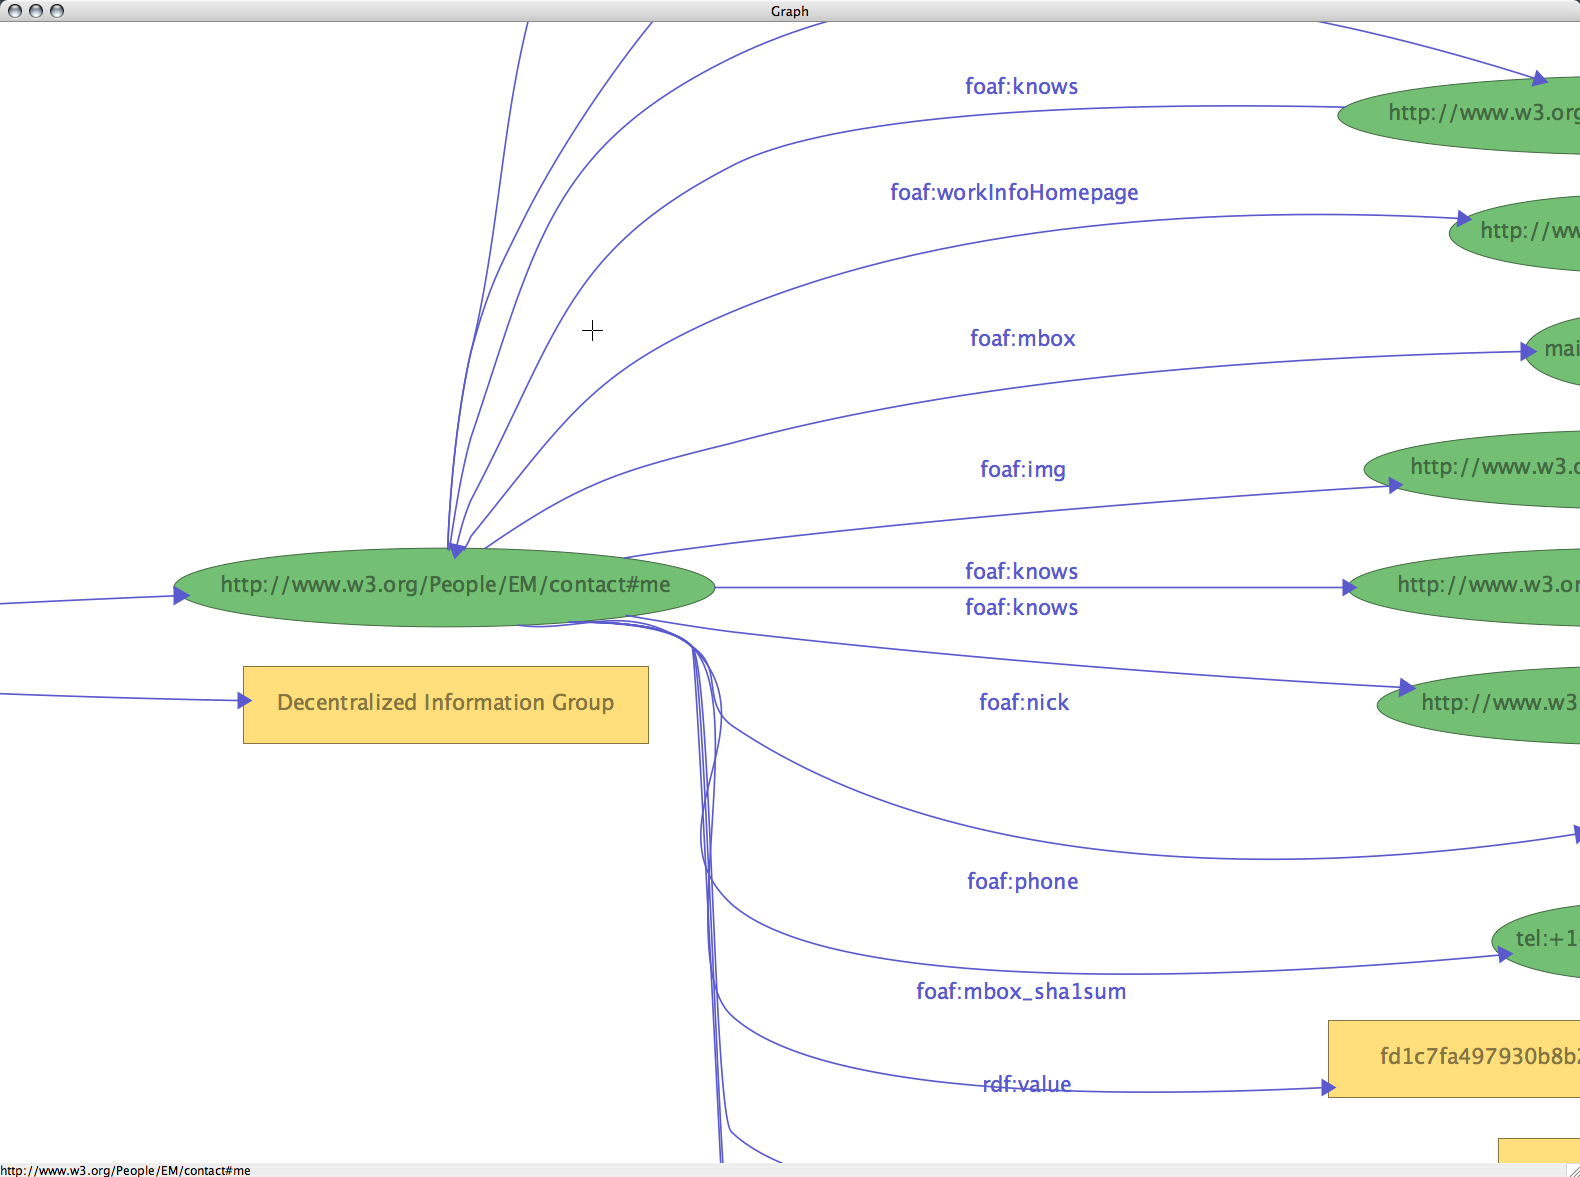
\includegraphics[height=4.45cm]{isavizscreen1.png} \hspace{0.04cm} &
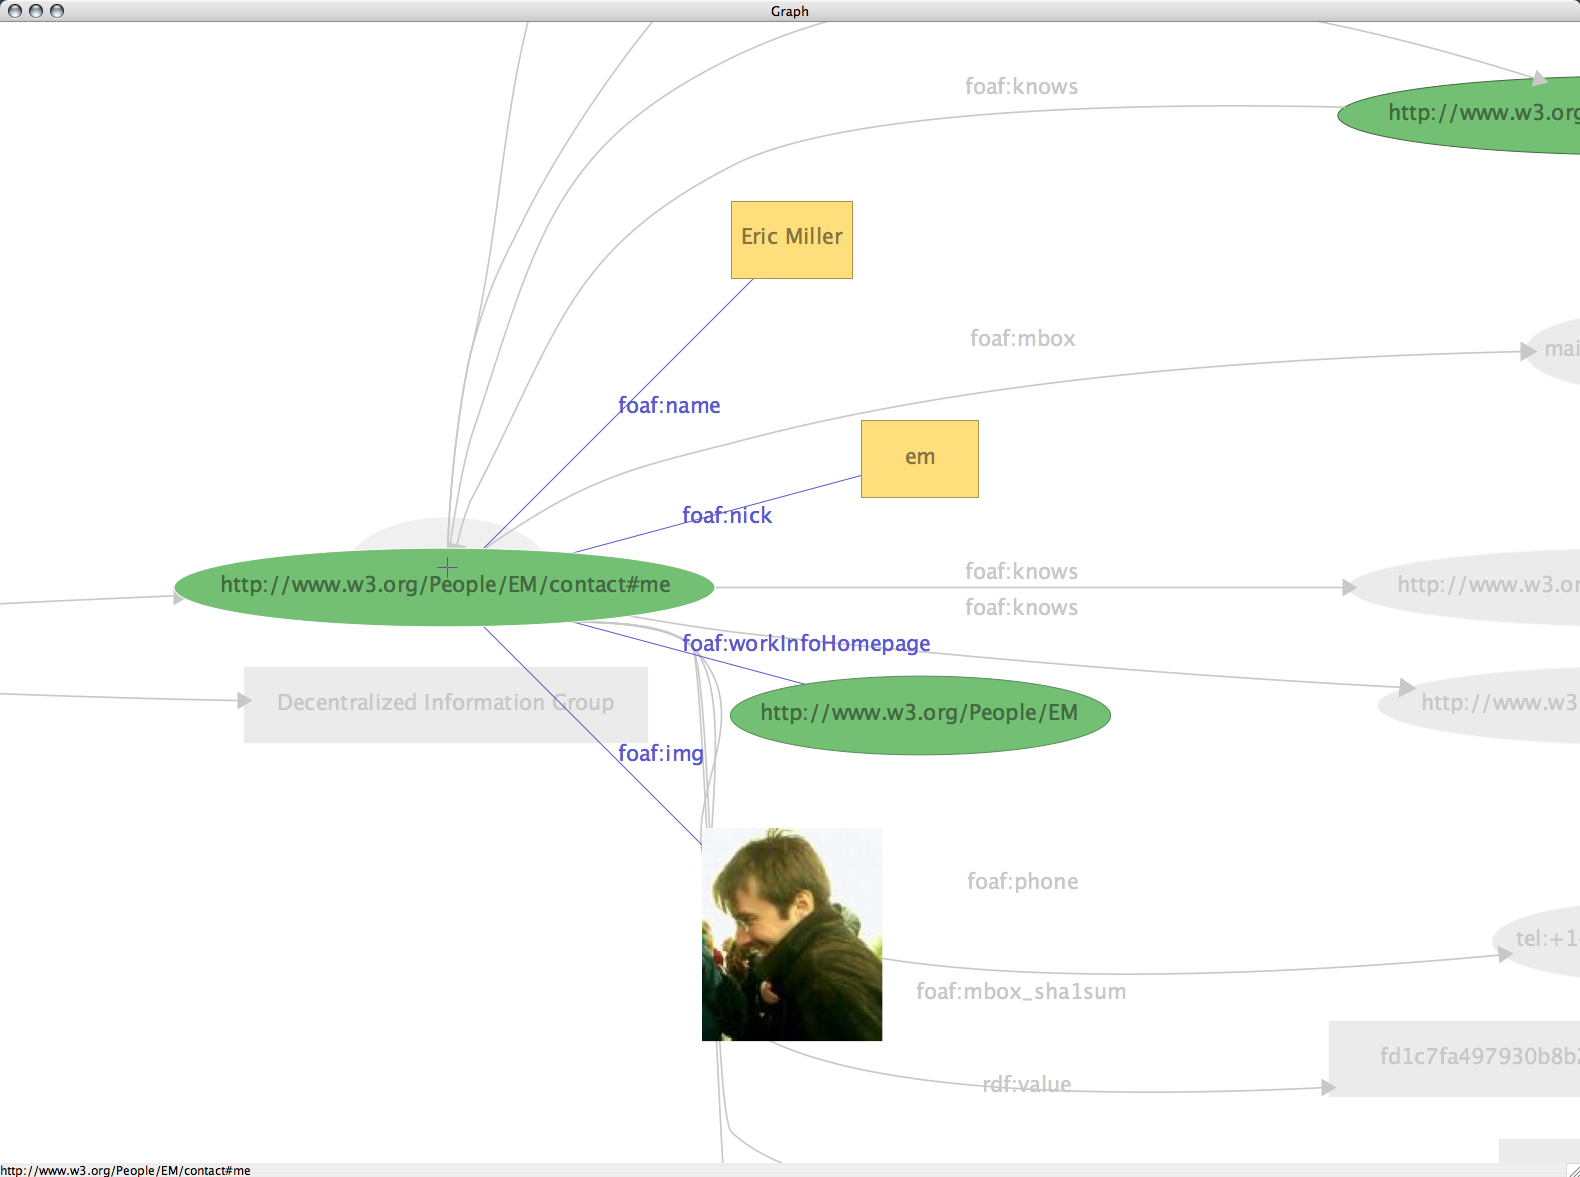
\includegraphics[height=4.45cm]{isavizscreen2.png} \\
\end{tabular}
\vspace{-1em}
\caption{Zoomed-in view of a \rdf{foaf:Person} resource in IsaViz: default presentation (left) and rendered with a Fresnel lens (right)}
\label{isvFresnelFig}
%\vspace{-1em}
\end{figure}

Fresnel core formatting instructions are interpreted as customizations of the original layout and rendering of nodes and links in the diagram. For instance, nodes representing \rdf{foaf:image} property values can be rendered by fetching the actual image from the Web, as illustrated in Figure \ref{isvFresnelFig} (right). The default labels of nodes and arcs can be customized using \rdf{fresnel:label} instructions. In case a resource is the subject of multiple statements involving the same property or properties defined as \rdf{fresnel:mergeProperties}, the arcs and nodes representing these statements can be merged as a single arc and node with all values within that node, optionally separated by text as specified in \rdf{fresnel:contentBefore}, \rdf{fresnel:contentAfter} and related formatting instructions.


\vspace{1em}
{\bf Cardovan} is IBM's implementation of Fresnel lenses (see Figure \ref{cardovanFig}). Written in Java, Cardovan renders lenses with the SWT graphical user interface toolkit.  Cardovan is similar to other implementations in that it uses a subset of CSS to specify the layout of lens components on the screen. A remarkable feature of Cardovan is that it allows users to modify a lens in place. Users can add new properties to the lens, modify property values, and rearrange the physical layout of the properties displayed, though it is not a full WYSIWYG Fresnel lens designer. The project is still in its early stages, but is functional and is already being used for internal projects at IBM.

\begin{figure}
\begin{center}
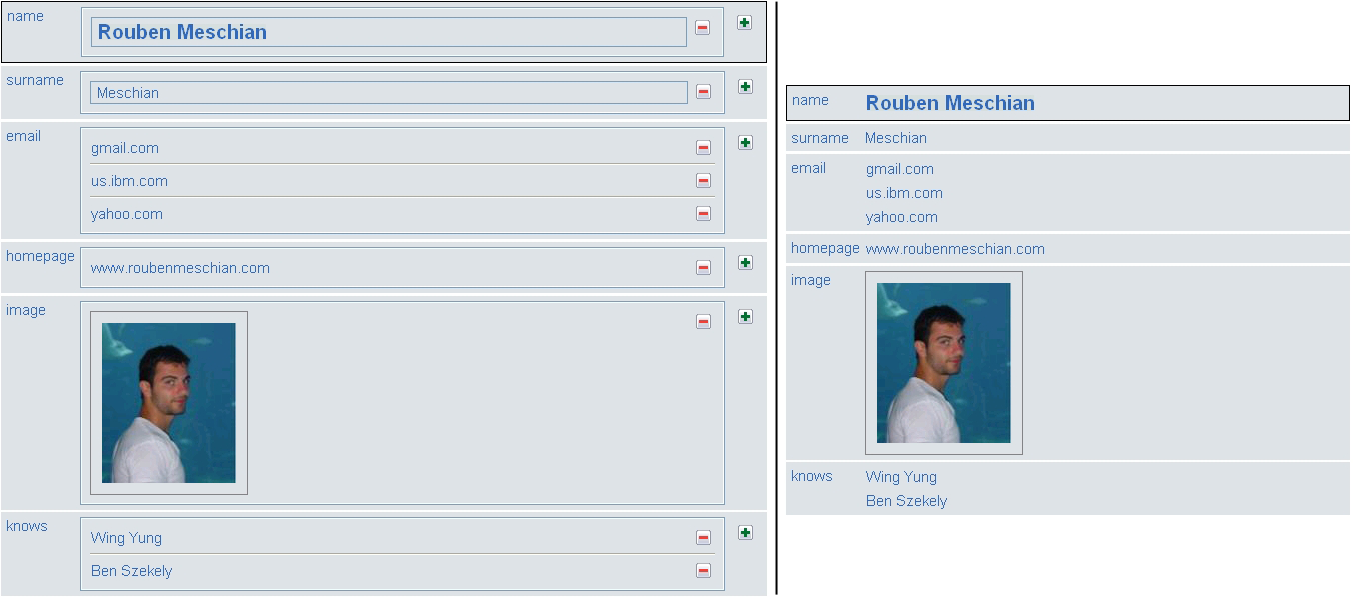
\includegraphics[width=12.2cm]{cardovan.png}
\end{center}
\vspace{-2em}
\caption{Editing a lens (left) and visualizing the result (right) in Cardovan}
\label{cardovanFig}
\end{figure}
